\chapter{The Solution}

I will discuss the design and implementation of each of the main components of the project separately.

\section{\tsPEG{}}

\subsection{High Level Design}

\tsPEG{} was built using the TypeScript PL. \tsPEG{} runs on the NodeJS JavaScript runtime. The NodeJS runtime allows us to execute JavaScript (and hence TypeScript) code locally.

The source code is hosted online at
\href{https://github.com/EoinDavey/tsPEG}{github.com/EoinDavey/tsPEG}, and the \tsPEG{} package is available on the NPM package repository at \href{https://www.npmjs.com/package/tspeg}{npmjs.com/package/tspeg}.

\tsPEG{} is self hosting, meaning that the input parser for \tsPEG{} was generated by \tsPEG{}. The software architecture of \tsPEG{} is given in Figure \ref{tspegdiagram}. The usage flow of using \tsPEG{} is as follows. First the user creates a grammar file, specifying the input grammar they want to generate a parser for. The syntax for the grammar file follows a similar pattern to the familiar EBNF syntax for grammar specification. In this file they specify the syntax rules, as well as names of AST fields, and computed properties. The \tsPEG{} binary is then called and it is passed in the grammar file.

\begin{figure}
    \caption{\tsPEG{} High Level Design}
    \label{tspegdiagram}
    \begin{center}
    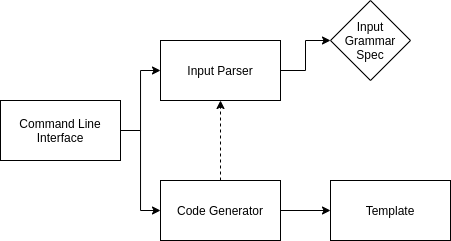
\includegraphics[scale=0.75]{tspegdiagram}
    \end{center}
\end{figure}

\tsPEG{}s own parser consumes the grammar file, and generates an internal description of the grammar. The code generator then takes this grammar specification and generates parsing functions for each rule, as well as TypeScript type declarations and classes for each of the AST nodes. These functions and types are then packaged up into a template file and then written to disk.

\subsection{Grammar specification}

\tsPEG{} uses a custom syntax to define grammars. Figure \ref{tspegexample} contains an example of a grammar specification for simple arithmetic expressions like "1+2*3".

\begin{figure}
    \caption{\tsPEG{} input grammar example}
    \label{tspegexample}
    \begin{lstlisting}
SUM  := head=FAC tail={ op='\+|-' sm=FAC }*
FAC  := head=ATOM tail={ op='\*|/' sm=ATOM }*
ATOM := val=INT
      | '\(' val=SUM '\)'
INT  := val='[0-9]+'
    \end{lstlisting}
\end{figure}

Grammars are defined by a sequence of grammar rules, for example
    \[\texttt{match} := \texttt{rule1} \mathbin{|} \texttt{rule2} \mathbin{|} \texttt{\textquotesingle a+\textquotesingle}\]
    defines a new rule \verb|match| that tries first \verb|rule1| then \verb|rule2|, then tries to match the regex expression \verb|a+|. The full list of operators is included in Appendix A.

    The \tsPEG{} grammar also allows specification of computed properties, for example Figure \ref{tspegcomputed} defines a rule to match integer literals that stores the value of the integer as a computed property.

\begin{figure}
    \caption{\tsPEG{} computed properties example}
    \label{tspegcomputed}
    \begin{lstlisting}
    INT := literal='[0-9]+'
           .value = number { return parseInt(this.literal) }
    \end{lstlisting}
\end{figure}

\subsection{Bootstrapping}

When developing \tsPEG{}, first a simple input parser was written by hand, supporting only the most basic syntax. A code generator was written that could take in the AST from this simple grammar and output a parser for it. Then the meta-grammar for the input grammar syntax was written and the generator was run. This replaced the hand written parser with a new generated one, self hosting itself and opening itself up to bootstrapping.

This new self hosting generator was then used to add more and more features and operators to itself, eventually resulting in the full self describing meta-grammar for the \tsPEG{} input syntax in Figure \ref{tspegsyntax}.

\begin{figure}
    \caption{\tsPEG{} meta-grammar definition}
    \label{tspegsyntax}
    \begin{lstlisting}
GRAM      := header=HDR? rules=RULEDEF+
HDR       := '---' content='((?!---)(.|\n))*' '---'
RULEDEF   := _ name=NAME _ ':=' _ rule=RULE _
RULE      := head=ALT tail={_ '\|' _ alt=ALT }*
          .list = ALT[] { return [this.head, ...this.tail.map((x) => x.alt)]; }
ALT       := matches=MATCHSPEC+ attrs=ATTR*
MATCHSPEC := _ named={name=NAME _ '=' _}? rule=POSTOP _
POSTOP    := pre=PREOP op='\+|\*|\?'?
            .optional = boolean { return this.op !== null && this.op === '?'}
PREOP     := op='\&|!'? at=ATOM
ATOM      := name=NAME !'\s*:='
           | match=STRLIT
           | '{' _ sub=RULE _ '}'
ATTR      := _ '.' name=NAME _ '=' _ type='[^\s\{]+' _ '\{'
    action='([^\{\}\\]|(\\.))*'
'\}'
NAME      := '[a-zA-Z_]+'
STRLIT    := '\'' val='([^\'\\]|(\\.))*' '\''
_         := '\s*'
    \end{lstlisting}
\end{figure}

\section{\Setanta{}} \label{setantasolution}

\subsection{High Level Design}
\Setanta{} is also written in TypeScript. The code structure of \Setanta{} allows it to be run as a local REPL through the NodeJS engine, but also in the browser. A high level architecture diagram is given in Figure \ref{setantadiagram}.

The \Setanta{} runtime uses the \tsPEG{} parser generator to generate its parser. Both the browser and CLI execution environments import the same interpreter and parser, but provide their own set of built-in functions. Each runtime environment passes some input text to the parser, the parser returns an AST or a syntax error object. This AST can then be passed to the interpreter with the relevant builtins. The interpreter can then be stopped and started asynchronously from the main executing thread.

\begin{figure}
    \caption{\Setanta{} High Level Design}
    \label{setantadiagram}
    \begin{center}
    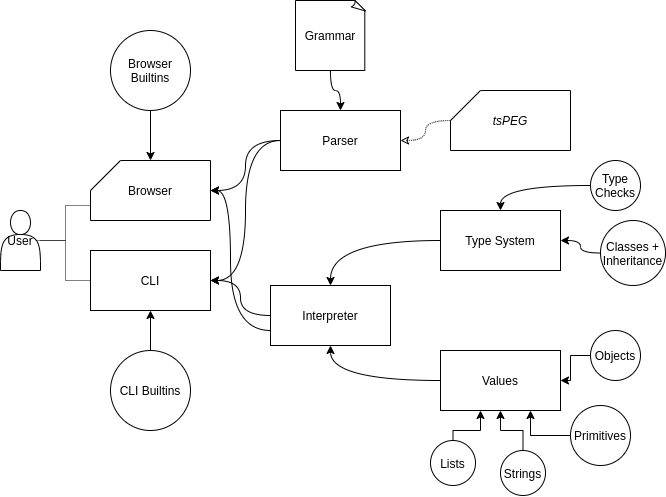
\includegraphics[scale=0.5]{setantadiagram}
    \end{center}
\end{figure}

\subsection{Syntax}

The syntax of \Setanta{} is new, but should feel familiar to most people. It has been designed to simple and approachable.

\Setanta{} programs, like most imperative languages, consist of a sequence of statements. Some important \Setanta{} features are outlined below:
\begin{itemize}
    \item \textbf{Variable declarations}

        In \Setanta{} variables are declared using the \verb|:=| operator, and can be re-assigned using the classic \verb|=| operator. The distinction is to provide a clear lexical difference between variable declaration and reassignment.
    \item \textbf{Loops + Conditionals}

        \Setanta{} support the classic conditional execution structure of if, else if, else. This is mostly a direct translation into Irish. However it should be noted that no bracketing is required around the expression.

            \begin{lstlisting}[language=setanta, frame=single, caption=Setanta conditionals]
má x == 0
    scríobh('Tá x cothrom le 0')
nó má x == 1
    scríobh('Tá x cothrom le 1')
nó
    scríobh('Tá x níos mo ná 1')
            \end{lstlisting}

            \Setanta{} supports two main types of loops, ``le idir'' loops that allow the user to specify start and ends to the loop, and ``nuair-a'' loops, which are the familiar while loops.

            \begin{lstlisting}[language=setanta, frame=single, caption=Setanta loops]
i := 0
le i idir (0, 10)
    i = i + 1
x := 0
nuair-a x < 10
    x = x + 1
            \end{lstlisting}
        \item \textbf{Classes + Functions}

            \Setanta{} supports declaring new classes, with methods, as well as functions on their own.
            \begin{lstlisting}[language=setanta, frame=single, caption=Setanta classes]
creatlach Person ó Animal {
    gníomh nua(name) {
        name@seo = name
    }
    gníomh speak() {
        scríobh('Hi, My name is ' + name@seo)
    }
}
            \end{lstlisting}
        \item \textbf{Literals}

            \Setanta{} supports literals for integers, booleans, null, strings and lists.
            \begin{lstlisting}[language=setanta, frame=single, caption=Setanta literals]
a := 500
b := 'Dia duit domhan'
c := [1,2,3,4, fíor]
d := fíor != breag
c := neamhní
            \end{lstlisting}
\end{itemize}

\subsection{The @ operator}\label{atoperator}

One of the most important features of \Setanta{}'s syntax is the @ operator. The @ operator is where the influence of the Irish language on the design of \Setanta{} is felt most clearly. In fact, the @ operator is a simple innovation that addresses 2 distinct differences between Irish and English.

The @ operator is the lookup operator, it is used to reference member fields and methods of objects. It is functionally equivalent to the classic dot ('.') operator in C, C++, Java, Python, JavaScript etc. The subtle difference is the order, both the @ operator and the '.' operator are binary operators, but the @ operator flips its arguments compared to the '.'.

In the standard usage of the dot operator, the expression \verb|a.b| refers to the member ``b'' of the object ``a''. In \Setanta{} \verb|a@b| refers to the member ``a'' of the object ``b'', the order has been reversed.

This change seems unimportant, however, it breaks 2 deep and subtle links between English and the standard way we look at OOP programming languages.

Firstly, as discussed in the technical background, English is an SVO language, meaning that in sentences, the subject comes first, then the verb, then the object. This property of English is directly reflected in the design of the classic dot operator.

The usage of the dot operator for member lookup gives rise to expressions like \verb|man.goTo(shop)|, or \verb|dbClient.query(q)|, these expression implicitly put the subject first, then the verb, then the object, directly mimicking the SVO structure of the host language.

By using the @ operator in \Setanta{} we instead get expressions like \verb|goTo@man(shop)| or \verb|query@dbClient(q)|, these expressions put the verb first, then the subject, then the object, reflecting the VSO structure of Irish. This subtle connection between a simple operator like '.' and the linguistic properties of English is not apparent.

There is a second connection between English and the lookup operation that is broken by the @ operator. In English when talking about possession relationships (``has-a'' relationships in database terms), we list the entities in decreasing order of possession, e.g.,
\begin{quote}
    The man's car door window pane
\end{quote}
The order of possession here is
\[man \rightarrow car \rightarrow door \rightarrow window \rightarrow pane\]

In direct contrast to this, in Irish we list possession in increasing order, meaning we start at the bottom of the possession relationship and work our way up. We would instead list
\[pane \leftarrow window \leftarrow door \leftarrow car \leftarrow man\]

This linguistic difference between Irish and English is again addressed by the @ operator. The standard '.' operator reflects the English language structure, \verb|man.car.door.window.pane|, but in \Setanta{} we use the Irish ordering \verb|pane@window@door@car@man|. This is another connection between English and the standard design of PLs that is easily overlooked.

\subsection{Semantics}

The semantics of \Setanta{} will be familiar to most users, it's an imperative, strongly dynamically typed language. \Setanta{} supports a gauntlet of modern features including first class functions, inheritance, event based concurrency, and automatic memory management. Although \Setanta{} is an imperative language, it does support a more functional style of programming as well.

\subsection{Allowing blocking operations}

As discussed in the technical background section, the JavaScript runtime, whether it be NodeJS or a browser, only allow usage of a single thread, and no blocking operations. However, writing \Setanta{} allows the user to use blocking functions. Figure \ref{blockingcomparison} shows a side by side comparison of equivalent programs in JavaScript and Setanta, it's clear that the Setanta program is much simpler due to allowing the program to block.

\begin{figure}[ht]
    \begin{minipage}[t]{0.45\textwidth}
        \begin{lstlisting}[language=javascript, caption=JavaScript]
setTimeout(() => {
    console.log('sleep1');
    setTimeout(() => {
        console.log('sleep2');
        setTimeout(() => {
            console.log('sleep3')
        }, 100);
    }, 100);
}, 100);
        \end{lstlisting}
    \end{minipage}\qquad
    \begin{minipage}[t]{0.45\textwidth}
        \begin{lstlisting}[language=setanta, caption=Setanta]
sleep(100)
scríobh('sleep1')
sleep(100)
scríobh('sleep2')
sleep(100)
scríobh('sleep3')
        \end{lstlisting}
    \end{minipage}
    \caption{Equivalent code in JavaScript + Setanta}
    \label{blockingcomparison}
\end{figure}

\subsection{Concurrency}

If you open the JavaScript console on any browser and enter \lstinline[language=javascript]|while(true){}| the browser tab will cease to be functional, i.e no buttons or text boxes or animations will work anymore. This is because the JavaScript engine is single threaded, the thread is busy computing \lstinline[language=javascript]|while(true){}|, and cannot process any other events.

In contrast, if you write \lstinline[language=setanta]|nuair-a fíor {}| in \Setanta{}, the browser tab will remain responsive. This is due to the implicit concurrency of all \Setanta{} functions. \Setanta{} manipulates the JavaScript engine task queue to ensure that execution time is shared between the main browser thread actions, and executing the \Setanta{} code.

\section{The learning environment - \trys{}}

\subsection{High Level Design}

\trys{}, like the other components is written mainly in TypeScript. The website is built on Google's LitElement library. LitElement is a library to write custom re-usable web components, it's a descendant of the Polymer framework, which has since been deprecated. LitElement is used to achieve a Material Design aesthetic. The text editor component uses the open source library CodeMirror.

The backend for \trys{} is written in Go, and runs on the Google App Engine (GAE) cloud infrastructure platform. The backend for the site supports the ability to save and retrieve \Setanta{} programs to the cloud.

A high level architecture for \trys{} can be seen in Figure \ref{trysetantadiagram}

\begin{figure}
    \caption{\trys{} High Level Design}
    \label{trysetantadiagram}
    \begin{center}
    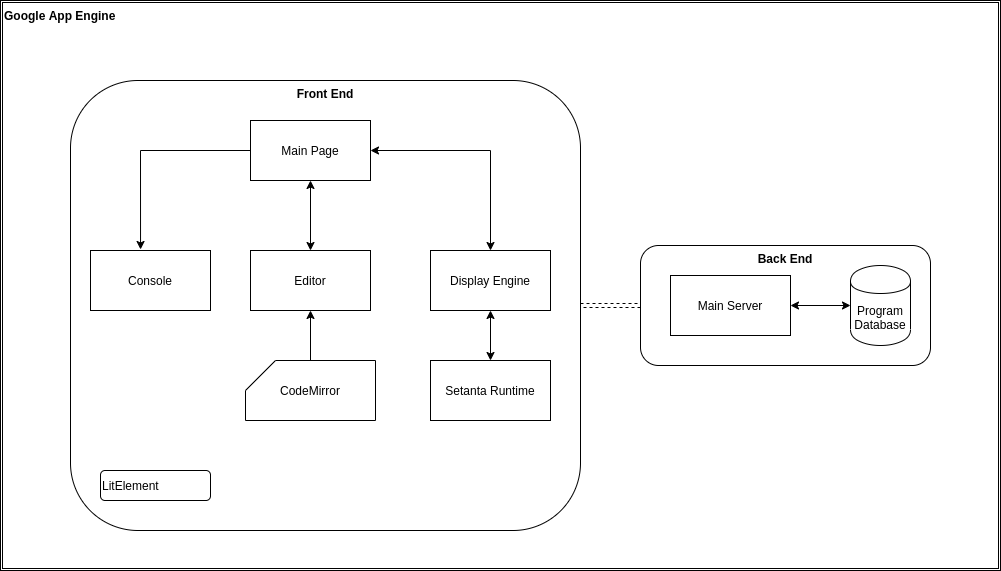
\includegraphics[scale=0.4]{trysetantadiagram}
    \end{center}
\end{figure}

\trys{} is known to work with the Google Chrome, Mozilla Firefox and Safari browsers, however it does not work with Internet Explorer, or older versions of Edge.

\subsection{Graphics API}

To better enable the educational experience on \trys{}, the \Setanta{} runtime has access to a graphics API. The graphics API allows the user to draw simple graphics primitives and animations. This API is exposed to the \Setanta{} program as a global object. The user can access various fields and methods on this object to draw and manipulate shapes on the display. Figure \ref{sierpinksitriangle} shows a short program on \trys{} that draws a Sierpinski triangle.

\begin{figure}
    \caption{Sierpinski Triangle draw with \Setanta{}}
    \label{sierpinksitriangle}
    \begin{center}
    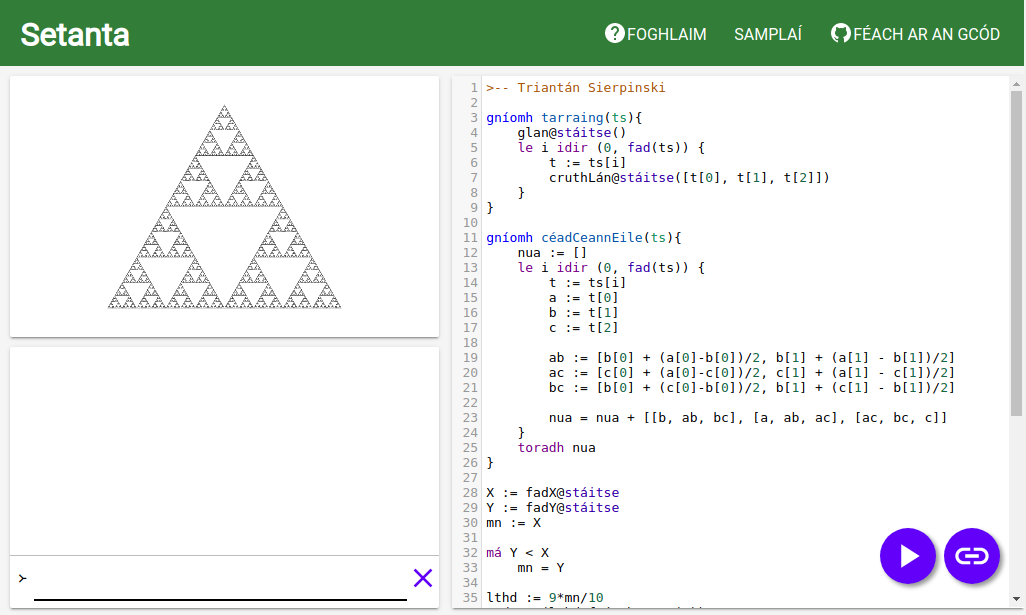
\includegraphics[scale=0.45]{sierpinskitriangle}
    \end{center}
\end{figure}

The graphics API also exposes methods to consume keyboard inputs, so the user can program simple games like \emph{Snake} with ease. It also features a full-screen mode.

\subsection{Saving Code}

\trys{} supports the ability to save a program to a specific URL. Clicking ``Faigh nasc'' (meaning ``get link'' redirects the user to a unique URL with which they can access their code. For example, the Sierpinski triangle example is available at:
\begin{quote}
    \href{https://try-setanta.ie/EhEKBlNjcmlwdBCAgIDgycODCg}{try-setanta.ie/EhEKBlNjcmlwdBCAgIDgycODCg.}
\end{quote}

This feature is handled by the Go backend on the Google App Engine. The programs are stored on the cloud Datastore, each program is identified by a unique integer. This unique integer is encoded into a string key, and this key is the URL where the code can be retrieved.
